\documentclass[10 pt,usenames,dvipsnames, oneside]{article}
\usepackage{../../../modelo-ensino-medio}



\begin{document}

\begin{center}
  \begin{minipage}[l]{3cm}

\includegraphics[width=2cm]{logo}    
\end{minipage}\hfill
\begin{minipage}[r]{.8\textwidth}
 {\Large \scshape Atividade: Expoentes inteiros}  
\end{minipage}
\end{center}
\vspace{.2cm}

\ifdefined\prof
%Habilidades da BNCC
\begin{objetivos}
\item \textbf{EM13MAT403} Comparar e analisar as representações, em plano cartesiano, das funções exponencial e logarítmica para identificar as características fundamentais (domínio, imagem, crescimento) de cada uma, com ou sem apoio de tecnologias digitais, estabelecendo relações entre elas.
\end{objetivos}

%Caixa do Para o Professor
\begin{goals}
%Objetivos específicos
\begin{enumerate}
\item Revisar as propriedades aritméticas das potências com expoentes inteiros;
\item Construir de modo intuitivo o significado de potências com expoentes inteiros negativos;
\end{enumerate}

\tcblower

%Orientações e sugestões
\begin{itemize}
\item Esta atividade tem um grande potencial para ser aplicada na forma de investigação. Separe a turma em grupos de no máximo $4$ alunos e peça que analisem os cartões em busca de relações e padrões, sem deixar que vejam as perguntas seguintes. Como se trata de um assunto supostamente conhecido por eles desde o Ensino Fundamental, espera-se que consigam perceber algumas relações importantes. Procure provocá-los com perguntas que levem-nos às propriedades das potências. Ao final, peça que socializem com os demais colegas as suas descobertas;

\item Espera-se que aqui ele solidifique a ideia de potência como produto de fatores repetidos, mas que perceba que não necessariamente ele precisa saber o resultado dessa operação para trabalhar com os objetos. Por outro lado, espera-se que ele extrapole essa ideia de multiplicação repetida ao lidar com expoentes negativos;

\item Chame a atenção dos estudantes para o fato de que ao lidar com expoentes negativos ampliamos a noção de potência de forma que a multiplicação repetida não é mais “a regra” ou a maneira correta de enxergar, ou seja, que $2^{-3}$ não é $2$ multiplicado por si mesmo $-3$ vezes. E que essa ampliação é feita de maneira que preserva as propriedades aritméticas já conhecidas.
\end{itemize}
\end{goals}

\bigskip
\begin{center}
{\large \scshape Atividade}
\end{center}
\fi

Observe os cartões abaixo, e responda às perguntas que seguem.

\begin{figure}[H]
\centering
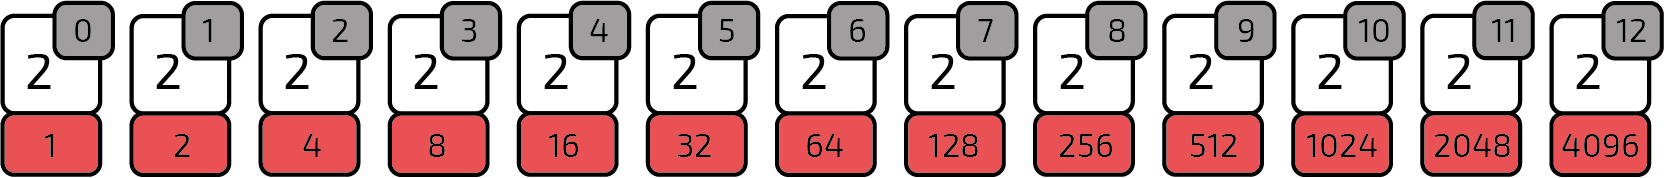
\includegraphics[width=.75\linewidth]{aritm1.png}
\end{figure}

\begin{enumerate}

\item{}
Que relação têm os números em um mesmo cartão?

\item{}
Que padrões se observam nos números em vermelho (embaixo) quando movemos para a \textbf{direita}? E nos números em cinza (acima)? Registre suas observações no esquema abaixo.

\begin{figure}[H]
\centering
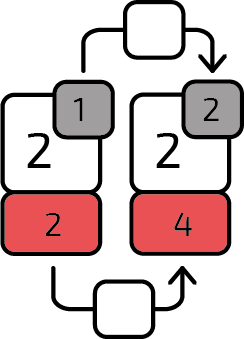
\includegraphics[width=65bp]{aritm2.png} \hspace{0,5cm}
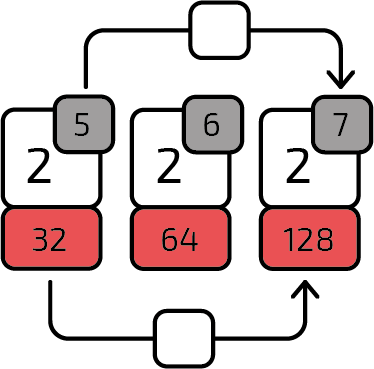
\includegraphics[width=90bp]{aritm3.png} \hspace{0,5cm}
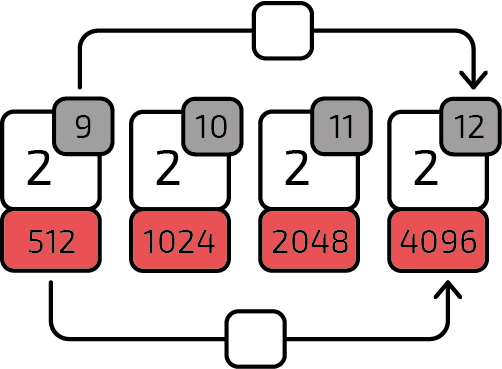
\includegraphics[width=120bp]{aritm4.png}
\end{figure}

\item{}
Complete o que falta no esquema abaixo. Escreva outros exemplos semelhantes e, então, generalize.

\begin{figure}[H]
\centering
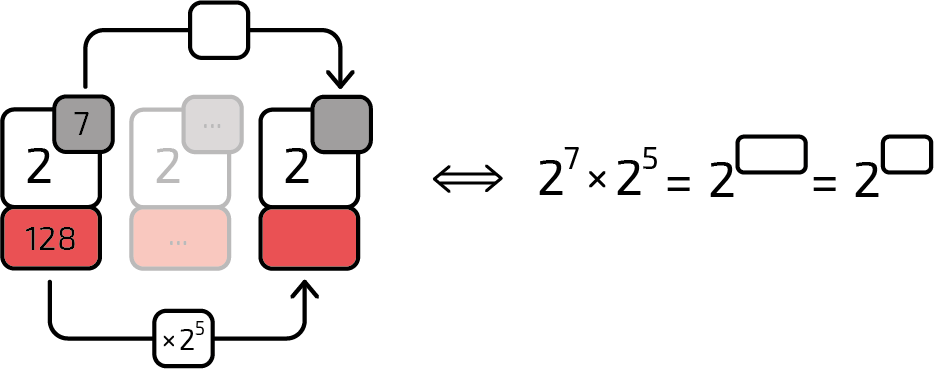
\includegraphics[width=200bp]{aritm5.png}
\end{figure}

\item{}
Que padrão se observa nos números em vermelho (embaixo) quando movemos para a \textbf{esquerda}? E nos números em cinza (acima)?

\begin{figure}[H]
\centering
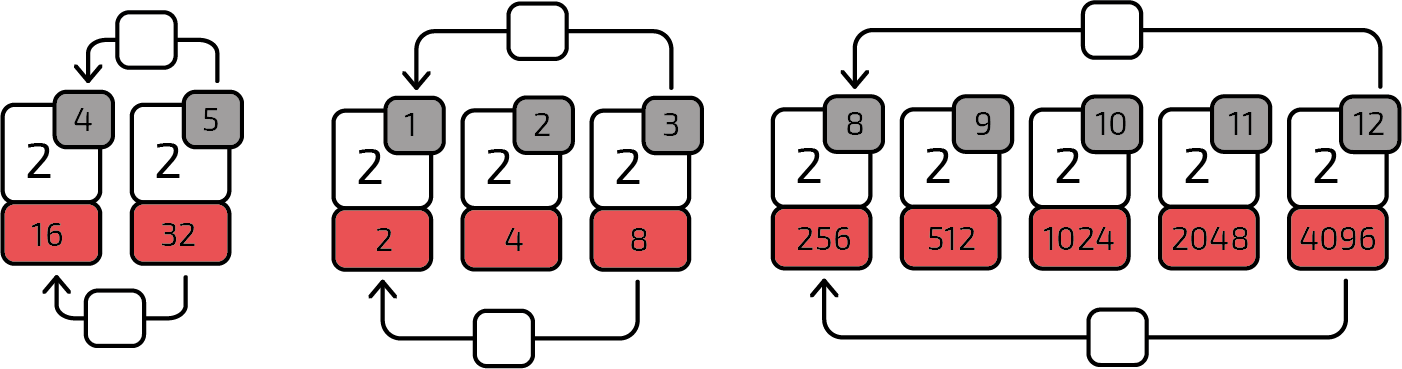
\includegraphics[width=280bp]{aritm6.png}
\end{figure}

\item{}
Complete o que falta no esquema abaixo. Escreva outros exemplos semelhantes e, então, generalize.

\begin{figure}[H]
\centering
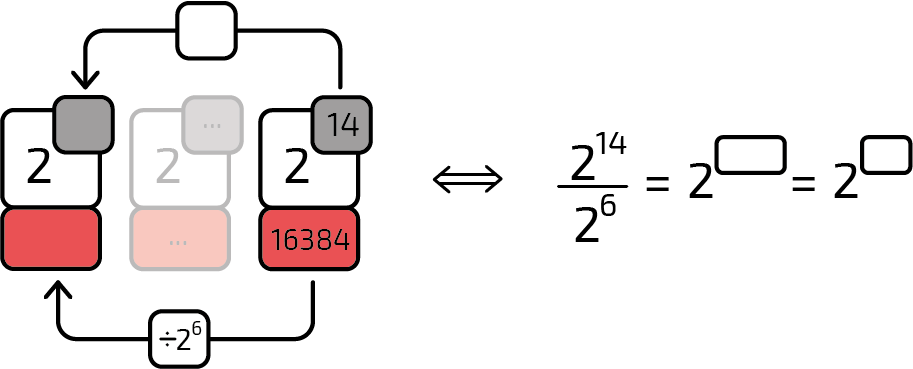
\includegraphics[width=220bp]{aritm7.png}
\end{figure}

\item{}
Proponha novos cartões, e explique suas escolhas.

\begin{figure}[H]
\centering
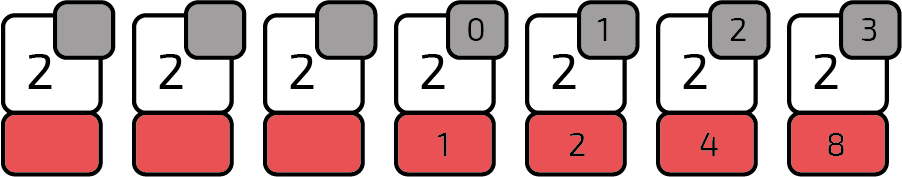
\includegraphics[width=200bp]{aritm8.png}
\end{figure}

\item{}
Baseado na sua proposta resolva.

\begin{figure}[H]
\centering
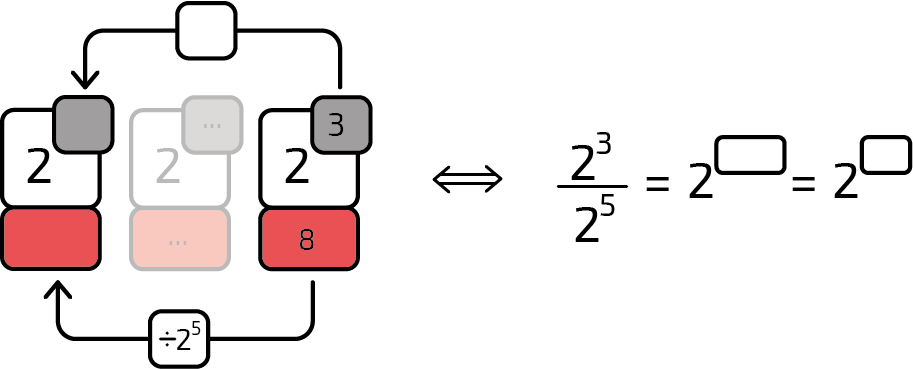
\includegraphics[width=200bp]{aritm9.png}
\end{figure}

\item{}
Complete o que falta no esquema abaixo. Escreva outros exemplos semelhantes e, então, generalize.

\begin{figure}[H]
\centering
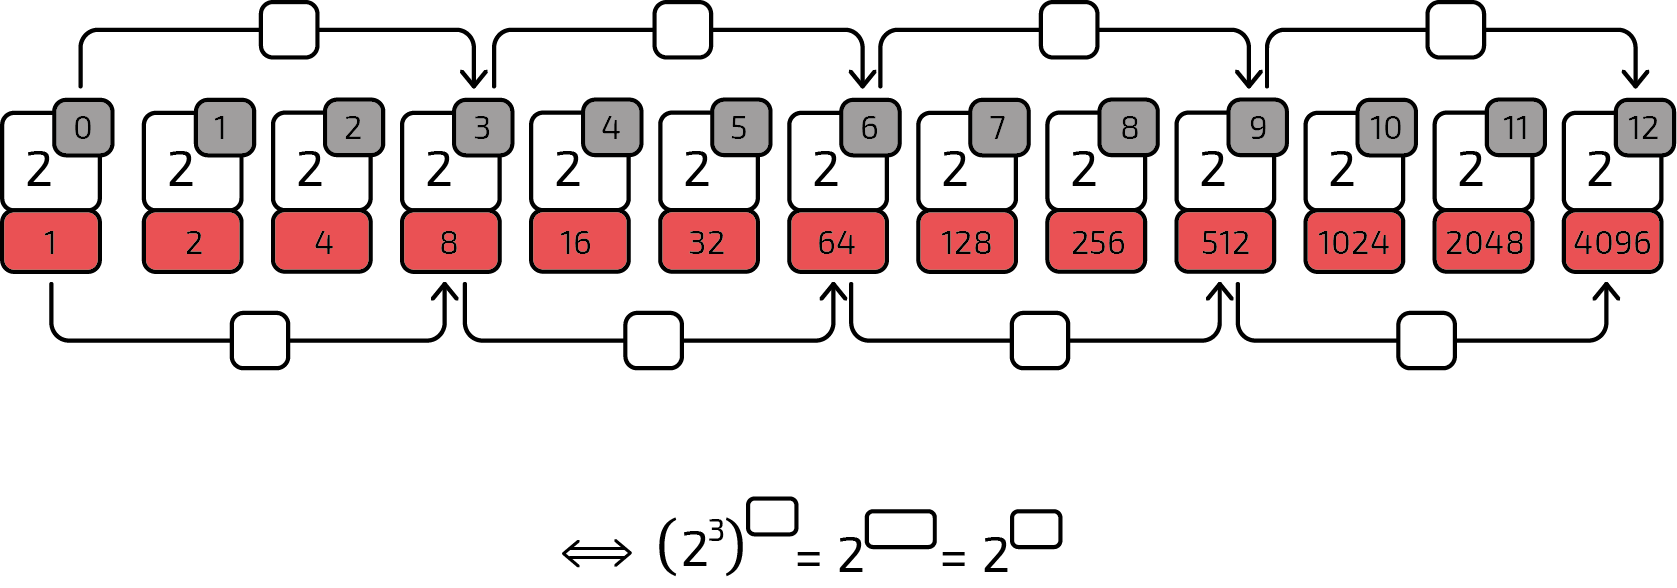
\includegraphics[width=300bp]{aritm10.png}
\end{figure}

\item{}
Sejam $m$ e $n$ números inteiros. Baseado nas suas conclusões nos itens anteriores, relacione a coluna da direita com a coluna da esquerda.

 (1) $2^{m} \cdot 2^{n}$  \hspace{1,0cm} (A) $2^{m \cdot n}$

 (2) $\dfrac{2^{m}}{2^{n}}$   \hspace{1,5cm} (B) $2^{m + n}$

 (3) $(2^{m})^{n}$  \hspace{1,1cm} (C) $2^{m - n}$

\end{enumerate}

\ifdefined\prof
\begin{solucao}

\begin{enumerate}
\item
O número $2$ elevado ao número em cinza é igual ao número em vermelho.

\item
Quando nos movemos de um cartão para o cartão seguinte a direita observamos que o número em vermelho é multiplicado por $2$ e o número em cinza aumenta uma unidade.

\begin{figure}[H]
\centering
\noindent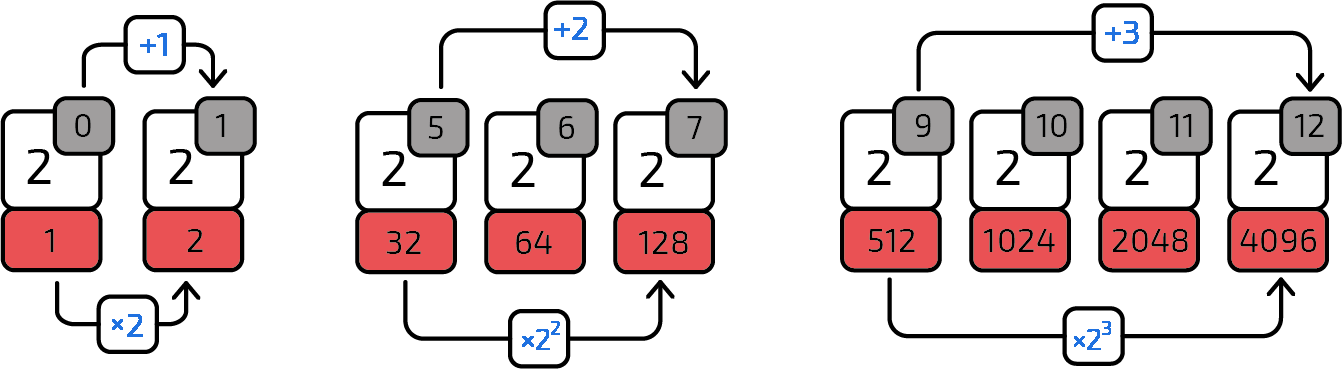
\includegraphics[width=.75\linewidth]{resp_inteiros_b.png}
\end{figure}

\item
O esquema será:

\begin{figure}[H]
\centering
\noindent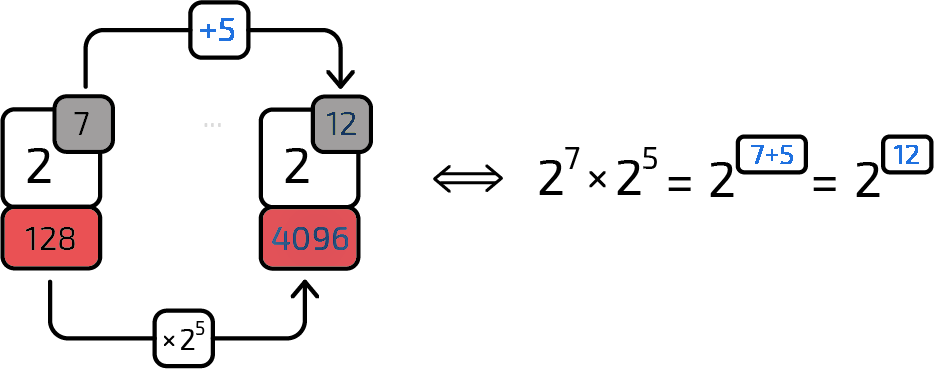
\includegraphics[width=.5\linewidth]{resp_inteiros_c.png}
\end{figure}

Alguns outros exemplos: $2^{9} \times 2^{4} =2^{9+4}=2^{13}$,\quad $2^{11} \times 2^8=2^{11+8}=2^{19}$. De um modo geral, se $m$ e $n$ são números inteiros então $2^m \times 2^n = 2^{m+n}$.

\item Quando nos movemos de um cartão para o cartão seguinte a esquerda observamos que o número em vermelho é dividido por $2$ e o número em cinza diminui uma unidade.

\begin{figure}[H]
\centering
\noindent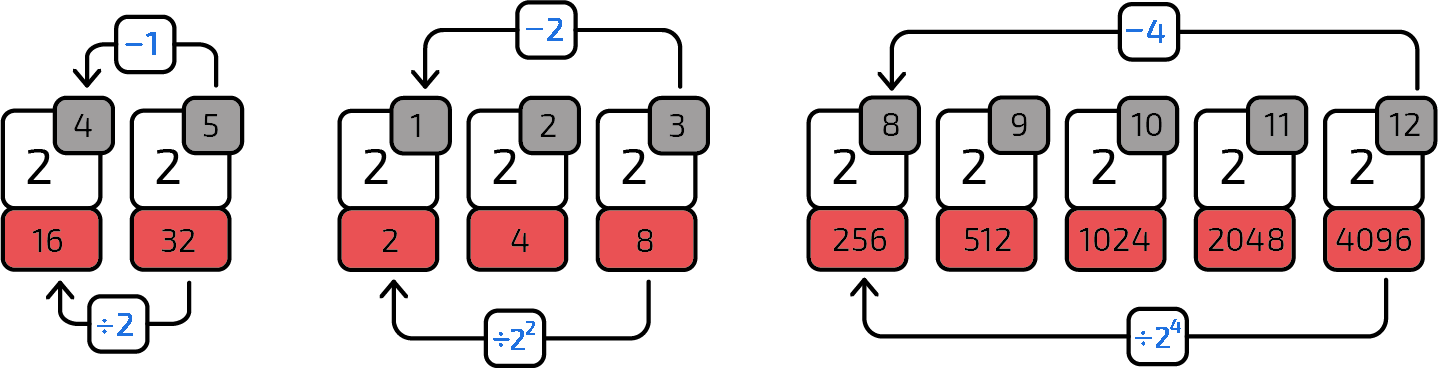
\includegraphics[width=.75\linewidth]{resp_inteiros_d.png}
\end{figure}

\item
O esquema será:

\begin{figure}[H]
\centering
\noindent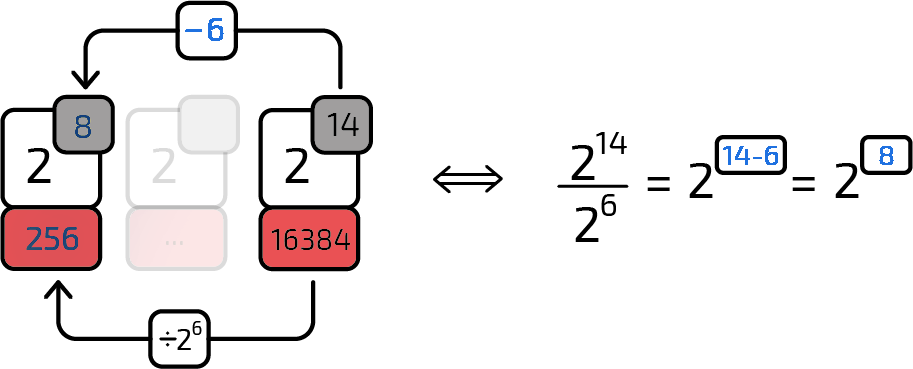
\includegraphics[width=.5\linewidth]{resp_inteiros_e.png}
\end{figure}

Alguns outros exemplos: $\dfrac{2^7}{2^5} =2^{7-5}=2^2$,\quad $\dfrac{2^{12}}{2^8} =2^{12-8}=2^4$. De um modo geral, se $m$ e $n$ são números inteiros então $\dfrac{2^m}{2^n} =2^{m-n}$.

\item Deverá ficar:

\begin{figure}[H]
\centering
\noindent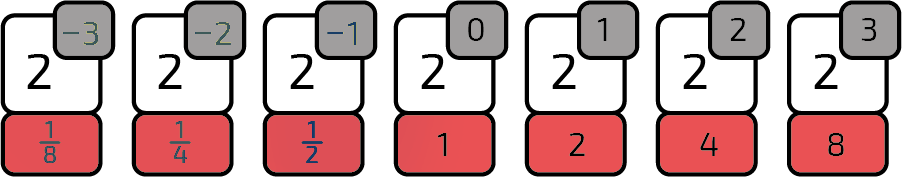
\includegraphics[width=.5\linewidth]{resp_inteiros_f.png}
\end{figure}

\item Teremos:

\begin{figure}[H]
\centering
\noindent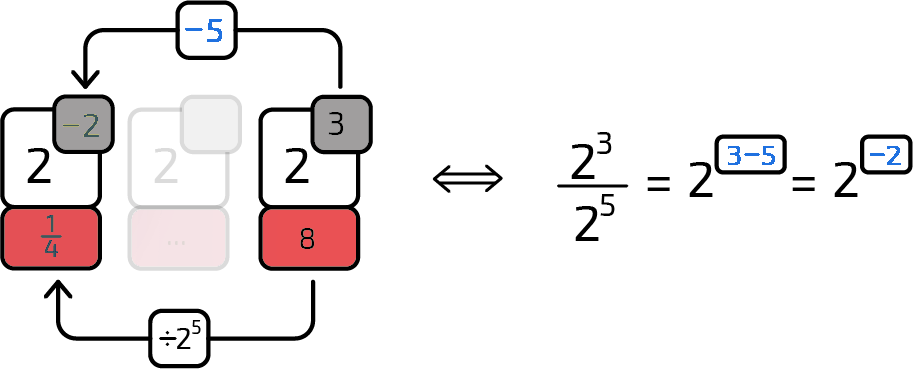
\includegraphics[width=.5\linewidth]{resp_inteiros_g.png}
\end{figure}

\item Completando o esquema vamos obter:

\begin{figure}[H]
\centering
\noindent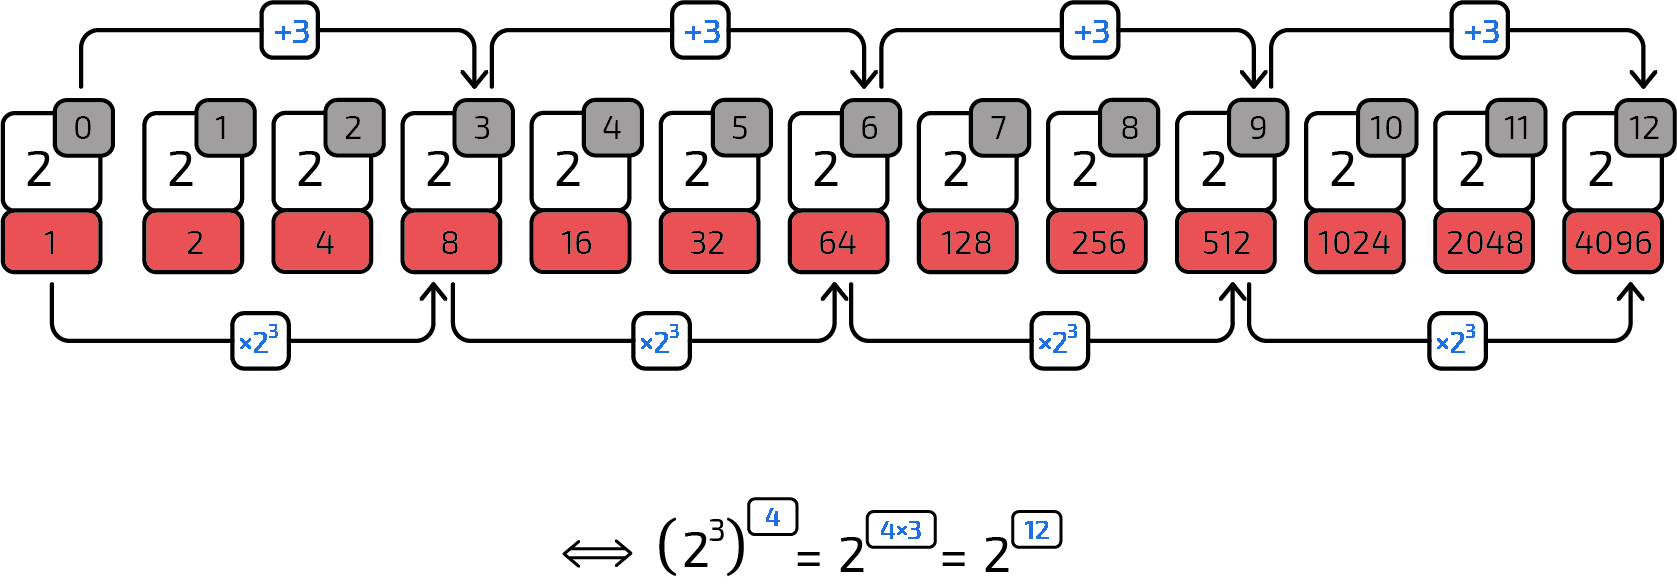
\includegraphics[width=.8\linewidth]{resp_inteiros_h.png}
\end{figure}

Alguns outros exemplos: $(2^{2})^{3}=2^{2\times3}=2^6$,\quad $(2^{8})^{5}=2^{8\times5}=2^{40}$. De um modo geral, se $m$ e $n$ são números inteiros então $(2^{m})^{n}=2^{m \times n}$.

\item (1)-(B),\quad (2)-(C),\quad (3)-(A).
\end{enumerate}


\end{solucao}
\fi

\end{document}